\documentclass{bioinfo}
\copyrightyear{2012}
\pubyear{2012}

\begin{document}
\firstpage{1}

\title[Pathway-based visualization of cross-platform microarray datasets]{Pathway-based visualization of cross-platform microarray datasets}
\author[Clemens Wrzodek \textit{et~al}]{Clemens Wrzodek\,$^{1\footnote{to whom correspondence should be addressed}}$, Johannes Eichner\,$^{1}$ and Andreas Zell\,$^1$}

\address{$^{1}$Center for Bioinformatics Tuebingen (ZBIT), \\University of Tuebingen, 72076 T\"ubingen, Germany}
\history{Received on XXXXX; revised on XXXXX; accepted on XXXXX}

\editor{Associate Editor: XXXXXXX}

\maketitle

\begin{abstract}

\section{Motivation:}
Text Text Text  Text Text Text Text Text Text Text Text
Text  Text Text Text Text Text Text Text Text Text  Text Text Text Text Text Text Text Text Text  Text Text Text Text Text Text Text Text Text  Text Text Text Text Text Text Text Text Text  Text Text Text Text Text Text Text Text Text  Text Text Text Text Text.

\section{Results:}
Text  Text Text Text Text Text Text Text Text Text  Text Text Text Text Text Text Text Text Text  Text Text Text Text Text Text Text Text Text  Text Text Text Text Text Text

%\section{Availability:}
%The described method is included in the InCroMAP application, which is available at \href{TODO}{TODO}.

\section{Contact:} \href{clemens.wrzodek@uni-tuebingen.de}{clemens.wrzodek@uni-tuebingen.de}
\end{abstract}

\section{Introduction}

The first generation of microarray platforms was developed as a high-throughput technique for
profiling the transcriptome of diverse biological systems (i.e., cells, organs or organisms) under
various experimental conditions (TODO: Refs. Golub, etc.). As these traditional gene-centered arrays
were mostly limited to mRNA transcripts, the vast majority of visualization tools are still focused
on mRNA datasets (Refs.). To date, a plethora of different microarray platforms are readily
available. These include gene-centered platforms which rely on current genome annotations as well as
unbiased tiling arrays which interrogate large non-repetitive regions of the genome. Diverse types
of platforms have been specificly designed for the interrogation of different genomic features,
ranging from mRNA or miRNA transcripts, through proteins or protein modifications, to relevant
functional elements such as exons, SNPs or promoters (TODO: Refs). In addition to arrays serving for
the quantification of global gene expression on the RNA or protein level, also epigenetic
modifications such as DNA methylation (DNAm) can be monitored on a genome-wide level using
microarray technology \citep{Hoheisel2006}.

% Motivation für die Entwicklung des Tools
Several tools exist for the visual inspection of datasets from individual platforms
(Refs.). However, the current inventory of publicly available tools, which are capable of
integrating and jointly visualizing data from multiple microarray platforms, is still very limited.
Here, we introduce a method, for integrated pathway-centered visualization of datasets generated
from the same biological samples using different microarray platforms, which interrogate
complementary genomic and epigenomic features.

% Pathway-basierte Visualisierung vs. Regions-basierte Visualisierung
In contrast to commonly used region-based visualization methods (e.g., \citep[see][]{UCSCBrowser},
TODO: weitere Beispiele und Zitate), we propose to visualize the microarray data in the context of
specific signaling or metabolic pathways, which can in many cases be more easily related to the
biological problem under study than individual genes or genomic regions.


% TODO: das h�chste der gef�hle sind methoden um 2 farben in 1 knoten, aber keiner kann DNA
% methylation oder sogar miRNA knoten rein.

% TODO: Johannes: Kannst du 1-2 S�tze jeweils zu Cytoscape, Ingenuity, eventuell noch Cytoscape +
% Plugins schreiben?

% TODO: Related Work. Abgrenzung zu GenMAPP und Ingenuity, Cytoscape, KEGG Atlas, KEGG Array; Siehe
% auch Kohlbacher-Nils Paper, S. Symons paper .Gibt es ueberhaupt ein Tool, welches alle 4
% Datentypen (miRNA, etc) visualisieren kann?

% TODO: InCroMAP vs. publizierte Pathway-basierte Visualisierungstools
There are other tools, specialized in pathway analysis (e.g., Ingenuity, ), or in pathway
visualization (Cytoscape, KEGG Atlas). Some even offer visualizing data in a pathway (GenMAPP, KEGG
Array, Symons programm). No method today for high-dimensional, heterogeneous cross-platform
datasets.

% Integrated oder single platform enrichment zur Identifikation der relevanten Pathways The pathways
which are relevant for the conducted experiment can be deduced from the differentially expressed
genes using pathway enrichment analysis. For this purpose, candidate pathways which are putatively
involved in the studied biological phenomenon are typically ranked according to p-values resulting
from a hypergeometric test for overrepresentation. The results are usually presented to the user as
a sorted table or barplot which does not show any superordinate relations of the pathways detected
as enriched with differentially expressed genes. In addition to this traditional approach, we also
implemented an alternative method, which provides the user with a more structured view of the
metabolic pathways linked to a certain microarray experiment. Owing to the hierarchical structure of
the KEGG PATHWAY database, InCroMAP can visualize the enrichments computed for each individual
metabolic pathway in the context of the higher-order overall metabolic pathway map compiled by KEGG
(http://www.genome.jp/kegg/pathway/map/map01100.html). Starting from either a ranked pathway table
or a colored meta-pathway map, individual pathways can be visualized in InCroMAP and overlaid with
microarray data from multiple platforms, to facilitate thorough visual inspection of the measured
pathway alterations. In contrast to previous work (TODO: Refs zu Cytoscape, Explain, etc.), InCroMAP
offers convenient functions to overlay a pathway plot with sample-matched microarray data from
platforms measuring gene regulation on mRNA, miRNA, DNAm and protein level.

%%%%%%%%%%%%%%%%%%%%%%%%%%%
% CELL CYCLE PICTURE
%%%%%%%%%%%%%%%%%%%%%%%%%%%
\begin{figure}[tb]
\centering
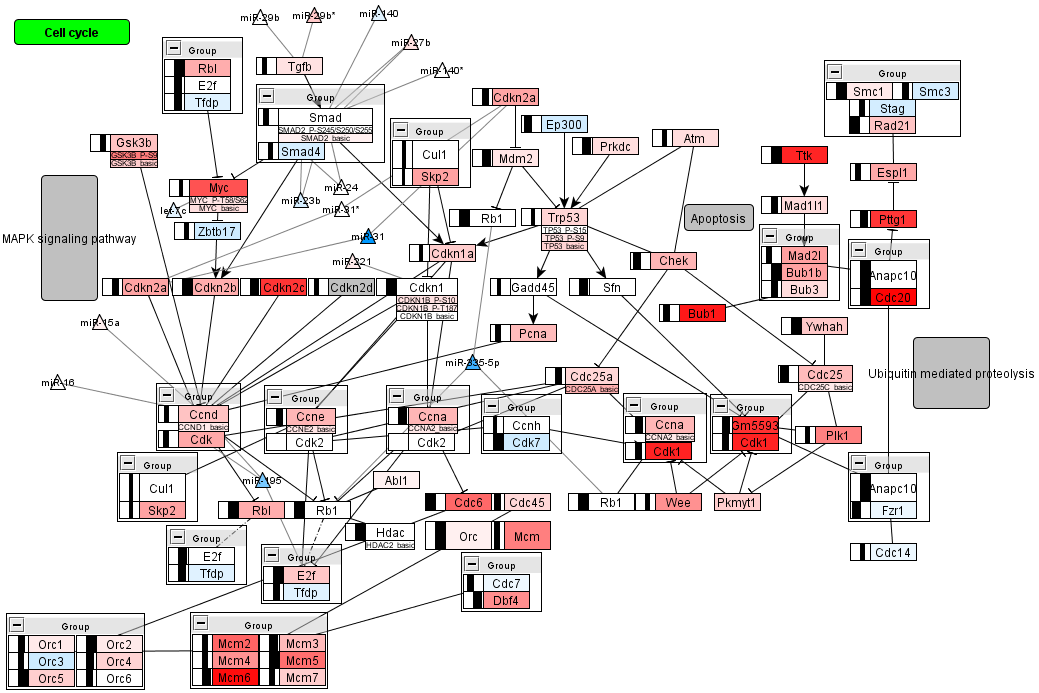
\includegraphics[width=.5\textwidth]{figures/mmu04110.png}
\caption{
TODO: Bild zeigt Cell Cycle pathway}\label{fig:cellcycle}
\end{figure}
%%%%%%%%%%%%%%%%%%%%%%%%%%%
%%%%%%%%%%%%%%%%%%%%%%%%%%%

%\begin{methods}
\section{Methods}

% Import von Microarray-Daten in InCroMAP
Before use with InCroMAP the microarray datasets of interest have to be preprocessed and annotated
using platform-specific workflows (Refs zu Ringo, MEDME, AgiMicroRna, Limma, Annotate). These
workflows usually involve (1) the quality control of the raw data (TODO: cite arrayQualityMetrics,
simpleaffy, etc.), (2) the data normalization to correct for background noise and experimental
variation (TODO: cite RMA and GCRMA paper or review paper about normalization), and (3) the mapping
of the probes to genes or genomic regions. After these preprocessing steps the microarray data has
to be exported in tabular format (e.g., CSV or Excel). These tables have to contain two types of
columns: (1) annotation columns, containing probe or probeset IDs (e.g., Affymetrix IDs) and
database IDs of the corresponding genes (e.g., Ensembl or Entrez IDs), and (2) data columns
containing either fold-changes and/or p-values resulting from basic statistical analysis of the 
microarray data.

% JE: Habe das mal rausgenommen, da es zu InCroMAP-spezifisch ist oder ?
% For convenience, these tables can be imported into InCroMAP per drag-and-drop, and the 
% tool tries to auto-detect the platform type.  

% Import von Pathways in InCroMAP 
The pathway data is automatically imported from KEGG. In the KEGG PATHWAY database each pathway map
is available for download as a KGML document which is internally converted into a GraphML document
by InCroMAP. These GraphML files can be interactively visualized by InCroMAP using the yWorks graph
viewer (TODO: Ref.). In order to overcome limitations of the KGML format, one can create an overlay
graph that shows the original KEGG pathway image in the background, which may provide the user with
additional information about cellular structure and compartmentalization.

% Visualisierung von Microarray-Daten im Kontext von Pathways
After uploading the data, the KEGG pathway nodes, which correspond to genes or gene families, can be
overlaid with fold-changes measured on mRNA or protein expression level. Furthermore, DNA
methylation changes observed in the proximal promoter regions can be visualized. In the final step,
additional nodes corresponding to miRNAs can be added to the pathway and colored according to the
expression changes measured in the underlying experiment. See Figure~\ref{fig:visualization_steps}
for an illustration of all the above-mentioned visualization steps.

\subsection{Pathway visualization}

The basic prerequisite for generating a pathway-based visualization is visualizing the pathway
itself. For this purpose, we are using KEGGtranslator \citep[see][]{Wrzodek2011}, which performs a
basic conversion of the KEGG KGML documents to GraphML and to annotates all nodes with EntrezGene
identifiers (Ref. zu NCBI EntrezGene). In short, KEGGtranslator converts all KGML entries to nodes
and all relations to edges. Some basic errors are corrected automatically and appropriate shapes,
colors and labels are inferred. Then, all nodes are annotated with diverse identifiers,
descriptions, and further information. The resulting document provides the basis for the
subsequently generated visualizations.

% JE: Die Bedeutung von den KEGG-Knoten (einzelne Gene oder Genfamilien) habe ich weiter oben eingebaut. 
% Ich würde daher den folgenden Absatz streichen um den Leser nicht zu ausführlich mit Details vollzulabern ;-)
% 
% At this point, it is important to note that KEGG usually draws referenced
% pathways as rectangular nodes with rounded corners, small molecules as circles, and single gene
% products (e.g., enzymes) as well as gene families as rectangles. This means that one rectangular
% node can consist of multiple different enzymes, depending on the KEGG definition.

% Vorteile des Pathway-Bilds im Hintergrund
At least for some pathways the KGML document available at KEGG does not contain all information 
displayed in the corresponding pathway map. Thus, an overlay graph can be generated which contains the 
original pathway map as a static transparent image in the background of the interactive graph plot 
(see Figure~\ref{fig:visualization_steps}b). Owing to this feature, additional information on 
cellular structure (e.g., schematic drawings of receptors involved in cell signaling) can be maintained. 
This feature also enhances the visualization of the global maps in KEGG PATHWAY, as additional
information on the organisation of subordinate pathway groups is provided by the pathway image.

\subsection{Visualization of messenger-RNA expression data} 

% Darstellung von mRNA-Daten
As mRNA expression data is typically available for the whole genome, and thus also for the majority
of nodes in a particular KEGG pathway, these data are displayed in the background color of the
nodes.

% Eingabeformat für mRNA-Daten
As input our method requires preprocessed mRNA datasets with annotation columns (e.g., probeset and
gene identifiers) and data columns, which are referred to as \emph{observations}. In this context,
observations can be any statistical significance (e.g., \emph{p}-values) or comparative measure
(e.g., fold-changes or log-ratios).

% Mapping von mRNA-Daten auf Pathway-Knoten
Next, these data have to be broken down to a single value for each pathway node, which then
corresponds to the color of the node.  As single nodes can represent multiple genes in KEGG, the
intensities measured by probes, corresponding to the same node, have to be summarized. To this end,
the mean or median is calculated across probes, which were mapped to the same node, or the probe
with the strongest or most significant signal (i.e., $\min\emph{p}-value$ or $\max|fold-change|$) is
adopted for coloring the node.

% Einfärbung der Knoten
To visualize fold-changes or log-ratios in the context of pathways a color gradient ranging from
blue to red is used to illustrate down- and upregulation, respectively. Non-differentially expressed
genes are shown in white, and pathway nodes for which no mRNA data is available are displayed in
grey. If desired \emph{p}-values can be shown instead of fold-changes. For this purpose, we propose
to map the negative logarithmized \emph{p}-values to a color gradient, which leads to a more
intuitive illustration of the observed significances.  See Figure~\ref{fig:visualization_steps}c)
for an example of visualized mRNA data.

% JE: Würde den Absatz streichen, da er zu viele technische Details enthält  
% For fold-changes (which are usually $log_2$ values), we color every node with a fold-change $\geq2$ red
% and all fold-changes $\leq-2$ blue. Fold-changes of zero are defined to have a white color and
% colors between $\pm2$ are faded from blue or red to white, depending on the actual fold-change. The
% same procedure can be used for \emph{p}-values, except that just one minimum threshold and one
% minimum color must be defined. Furthermore, the color for \emph{p}-values should not be changed on a
% linear, but on a log-scale. 

\subsection{Visualization of protein expression data}

% Darstellung von Protein-Daten
Visualization of protein datasets is performed by adding small boxes below pathway nodes and
changing the color of the boxes according to the corresponding protein expression data. As state-of-the-art 
experimental techniques (e.g., reverse-phase protein arrays, quantitative mass spectrometry) 
facilitate the distinction between different protein modifications (e.g., phosphorylated or 
acetylated forms of proteins) (TODO: Refs), multiple measurements may correspond to the same gene. 
In this particular case, the expression change observed for each individual protein form is represented 
as a separate box below the corresponding node. Each of these boxes is then labeled according to the 
respective protein form and colored based on the underlying expression data, as described previously 
for mRNA datasets.

% Eingabeformat für Protein-Daten
We require protein datasets to be annotated with database identifiers referring to proteins (e.g.,
UniProt IDs) or genes (e.g. EntrezGene IDs), which allows us to perform a straightforward mapping to
pathway nodes.

\subsection{Visualization of DNA-methylation data}

% Darstellung von DNAm-Daten


% Eingabeformat für DNAm-Daten


% Ein Wert nur als Hinweis, hier geht etwas 
% click gibt details?]. 
% fold-change wird zu box von -2 bis +2
% p-value im grunde ein bar-blot von 1 bis 0.00005 oder so...
% Einzelner Wert mit binning und $\frac{\sum\limits_{i=1}^n\log_2 x}{n}$, f�r fold-changes oder so
% peak detection m�glich und max. peak anzeigen.

\subsection{Visualization of micro-RNA expression data}

Visualizing micro-RNA (miRNA) datasets is not straightforward, because pathways usually do not
contain miRNAs. Pathway mainly consist of small molecules and enzymes, which are products of protein
coding genes. Therefore, to add miRNAs to a pathway, a connection must be established from miRNAs to
to protein-coding genes.

Biologically, miRNAs are small non-coding RNAs that regulate gene expression by binding to mRNA
targets and somehow inducing a degradation of the targeted mRNA \citep{Bartel2004}. The targets for
each miRNA must be known and there are several databases that contain information about
experimentally verified miRNA targets (e.g., miRecords \citep[see][]{miRecords}, miRTarBase
\citep[see][]{miRTarBase}, TarBase \citep[see][]{TarBase}) or predicted miRNA targets
\citep{Alexiou2009}. We use these miRNA target databases to perform the linkage between miRNAs and
pathways.

Pathway-based visualization of miRNA datasets is done by annotating all known targets to every miRNA
in the input dataset. Then all miRNAs that have targets in any pathway that should be visualized are
added to the pathway as small triangular nodes. The relation to the pathway is then established by
creating an edge from every miRNA to every target in the pathway. The triangular miRNA nodes
themselves are colored according to their expression, as described for mRNA.  This leads to an
integrated visualization that contains miRNA expression, miRNA target relation information and (if
also mRNA data is visualized) the expression of the targeted
mRNA. Figure~\ref{fig:visualization_steps}f) shows an example result of the described procedure.

%\end{methods}

\section{Results and discussion}

In this work, we present a novel visualization method to integratively visualize pathway interaction
information, miRNA target relations, DNA methylation data, mRNA, (phospho-) protein, and miRNA
expression data. Visualizing single datasets in pathways is a good first step that is also included
in other methods and applications. Actually, any dataset with gene identifiers and expression values
can be somehow visualized by changing node colors or other aspects of pathway nodes. Hence, it is
not very hard to visualize mRNA datasets. But visualization of phosphoprotein, microRNA or DNA
methylation datasets is not easy, because each datatype has its own characteristics.  %% PROTEIN For
phosphoproteins, one destroys the data if expression values for differen protein modifications
(i.e. phosphoforms) are merged. Hence, we add a separate box with its own visualized expression
value for every protein and protein modification to the pathway graph.  %% MicroRNA For MicroRNAs,
the general method with adding gene identifiers to datasets and mapping to the pathways does not
work at all, because miRNAs are not contained in pathways. We visualize miRNAs together with an
additional information: the miRNA target relation. By identifying protein coding genes, whose mRNAs
are targets of miRNAs, one can add the miRNAs to the pathways and connect them to the protein coding
genes by inserting edges to the corresponding targets.  %% DNA METHYLATION DNA methylation
microarray datasets are region-based and thus contain a huge number of probes and information. The
connection to protein coding genes is usually performed by defining a region around the
transcription start site (TSS) of a gene and assigning all probes in this region to the gene.  %For
example, with this procedure one can define that all probes within -2000 and +500 bps of a TSS are
most important for the regulation of this gene's expression.  But then, it is not recommended to
visualize all this information in the pathway. For example, it would be possible to create small XY
plots of the promoter region for every gene and add these pictures as small icons below each
node. But this would clutter the picture and destroy the clarity of it. Thus, we concluded that it
is most important to know if there are methylation changes in a promoter and maybe also if the gene
is rather hyper- or hypomethylated. The methylation details can then be inspected manually later
(e.g., the InCroMAP application provides a detailed XY plot of the DNA methylation if one clicks on
a pathway node). But the most important information in the first place is, if there are methylation
changes at all. And this can be expressed with various summarization methods and a small black bar
that grows with the amount of significant methylation changes in a gene promoter. 

An example for a KEGG pathway with visualized mRNA, miRNA, protein and DNA methylation data can be
seen in Figure~\ref{fig:cellcycle}. The visualization of multiple heterogenous datatypes can not be
performed with either a loss of information or a loss of clarity. Since these integrated pathway
visualizations should provide an overview, rather than a detailed listing of all possible
information, we tried to keep the clarity and summarize information wherever possible.  
% Especially when visualizing four different data types, this is important. Hence, we provide a
% TODO: Ein schoenes ende finden. 


% TODO: Gesamtkonzept und Ergebnisse / Bilder vorstellen
% - Beschreiben das auch recht viele definitionen drin sind (farben, thresholds, selection of miRNA target databases)
% - Beschreiben dass DNAm nur ein Hinweis ist wo man naeher nachschauen sollte
% - Link (URL) auf InCroMAP HIER oder in CONCLUSIONS ?

\begin{figure*}[t] \centering 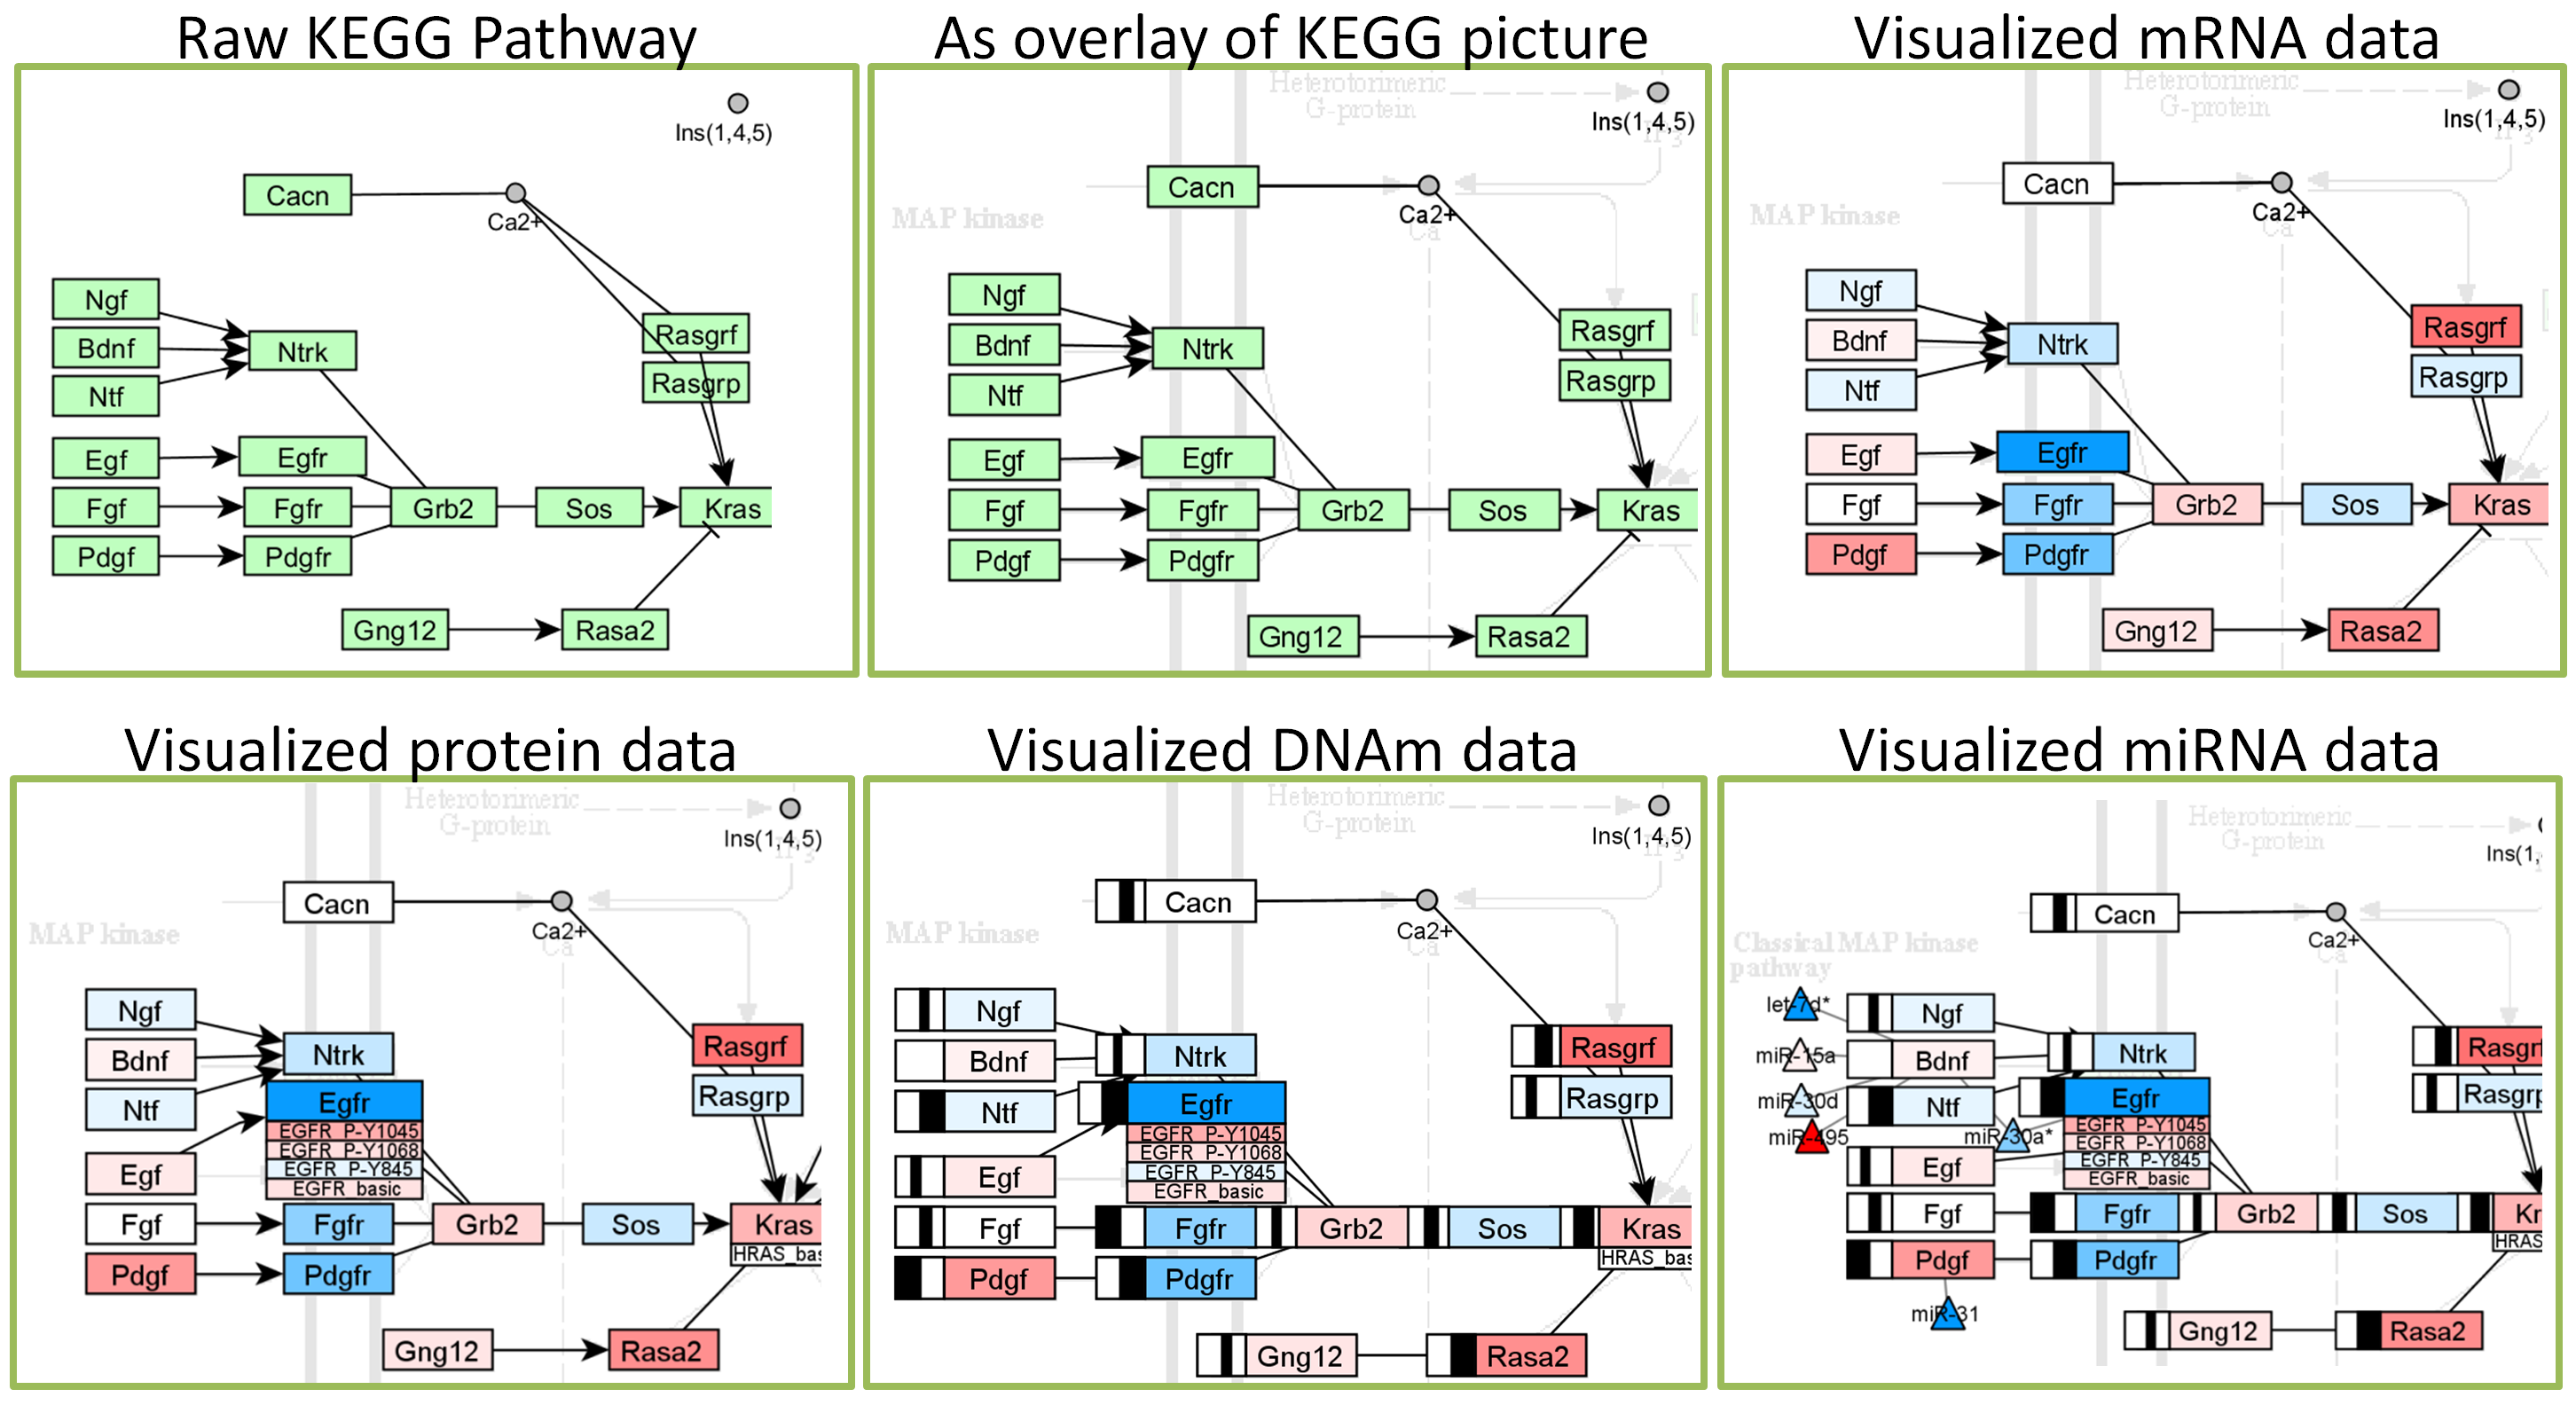
\includegraphics[width=1.0\textwidth]{figures/visualization-steps.png}
\caption{ TODO: Bild zeigt AUSSCHNITT des MAPK signaling pathway. Alle Schritte von a) bis f) kurz
          erlauetern und kurz sagen, dass f) quasi dem finalen Bild dieser Methode entspricht. }
\label{fig:visualization_steps} 
\end{figure*}


%TODO Abbildungen:
% - Sollen wie noch "Table 1" aus MARCAR D4.1 reinnehmen (tabellarische erklaerung der visualisierung aller 4 datentypen mit beispielen), und/oder
% - Ein schoenes Gesamtbild e.g. von cell cycle oder wnt signaling oder sowas
%[ - den metabolic pathway overview mit eingefarbten knoten] Dies nur wenn diese Methode auch noch bestandteil dieses papers wird (muesste noch bei methoden usw. aufgenommen und erklaert werden).


\section{Conclusion}

Pathway enrichment analysis is a common microarray data analysis tool to discover pathways, whose
genes show significant expression changes. In most applications, these enrichments are endpoints in
analysis workflows. There are some methods or applications that can show pictures of significantly
altered pathways and a few applications can even change node shapes or colors according to a single
expression dataset. However, not only the amount of available microarray datasets is growing
rapidly, but also the number of available platforms. Thus, today we have datasets that not only
consist of mRNA data, but also DNA methylation, miRNA, protein or even more different
levels. Analysis and especially visualization methods for such cross-platform datasets are very
rare.

Here, we present a pathway-based cross-platform microarray visualization method that is perfectly
suitable, e.g., as visualization method after pathway enrichment analyses. Especially the
visualization of DNA methylation and miRNA datasets is a feature that can not be found in other
visualization approaches. By integratively visualizing all datatypes, it helps researchers to
discover potential relationships across multiple layers. For example, a miRNA can be upregulated and
the corresponding mRNA target downregulated, whereupon a connected pathway protein could also be
downregulated in protein expression. This effect, which involves information about pathway relations
and miRNA targets, as well as miRNA, mRNA and protein expression, would be directly visible from the
here presented visualization method.

% TODO: - Zusammenfassung, vor allem Einzigartigkeit der Methode (insb. miRNA, (DNAm))
% herausstellen, - und kurze interpretation eines finalen bildes liefern ("man sieht in einem bild
% pathway informationen, miRNA relationen, expressionsdaten von miRNA, mRNA, bla; und sonst ist
% meist nach dem enrichment schluss bzw mRNA einfarbung bereits das maximum moegliche").

\section*{Acknowledgement}
We gratefully acknowledge contributions from Andreas Dr\"ager and Finja B\"uchel, as well as the
whole MACRCAR consortium.

\paragraph{Funding\textcolon}
The research leading to these results has received funding from the Innovative Medicine Initiative
Joint Undertaking (IMI JU) under grant agreement nr. 115001 (MARCAR project).

\bibliographystyle{natbib}
%\bibliographystyle{achemnat}
%\bibliographystyle{plainnat}
%\bibliographystyle{abbrv}
%\bibliographystyle{bioinformatics}
%\bibliographystyle{plain}

\bibliography{document}
%TODO: When paper is ready, comment \bibliography line and add content of document.bbl here.

\end{document}
